
\section{Introduction}


\section{Methodology}


\subsection{Forecast models}

Different forecast models have been developed for different types of data. 

In \cite{aggarwal2009electricity} a taxonomy of forecast models used for electricity price forecasting has been presented (Figure \ref{classification_of_price_forecasting_models2}). 

\begin{figure}[htbp]
	\centering
		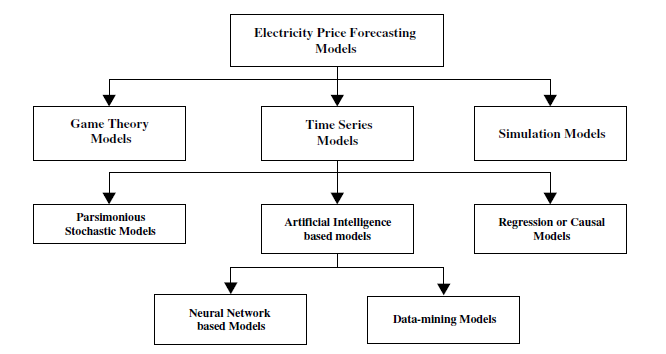
\includegraphics{figures/state_of_the_art/classification_of_price_forecasting_models.PNG}
	\caption{Classification of price forecasting models \cite{aggarwal2009electricity}}
	\label{fig:classification_of_price_forecasting_models2}
\end{figure}

Neural network models are best used to model complex and possibly unknown characteristics in the data where the model maps input to output data via a set of trained functions. 


%Ideas
%\begin{itemize}
	%\item explain periodogram in detail
	%\item seasonal decomposition (pg 41)
%\end{itemize}

\subsection{Seasonality estimation and periodogram}

Estimating seasonality is an important pre-processing step when building forecasting models. As most models are not able to automatically detect seasonality in the given data it is vital to determine possible seasonality cycles beforehand. 

One way of detecting seasonality in the data is by doing a spectral analysis for exploration of cyclical patterns. 
During the process the data is decomposed into underlying sinusoidal (sine and cosine) functions with particular wavelengths \cite{weron2007modeling}. 
The wavelength is commonly described as frequency which is the number of cycles per unit time. 

The frequency $\omega$ and the period $T$ have a reciprocal relationship $\omega = \frac{1}{T}$. Thus the period $T$ denotes the number of unit time stamps required to complete one period which in case of daily seasonality in a time series of hourly observations can be 24 hours. 

In order to visualize common frequencies a \textit{periodogram} may be generated which can be regarded as a tool for retrieving the most common frequencies from the dataset. As existing seasonality patterns in the data are likely to be detected by the periodogram as high valued frequencies it can be used to extract these frequencies and calculate the reciprocal as the seasonality period $T$. 

The formula of a periodogram for a vector of observations $\{x_1,\ldots,x_n\}$ is defined as \cite{weron2007modeling}:

		\[ I_n (w_k) = \frac{1}{n} \left| \sum_{t=1}^{n}{x_t  e^{-i(t-1) \omega_k} } \right|^2 \]
		
		where $\omega_k = 2 \pi (k/n)$ are the Fourier frequencies in radians per unit time, $k = 1,\ldots,[n/2]$ and $[x]$ denotes the largest integer less than or equal to $x$. 

Figure \ref{fig:periodogram_July_2014} shows a periodogram of two weeks of hourly day ahead prices where two frequencies are clearly visible in the diagram. These frequencies have values of $\omega_1 = 0.0416$ and $\omega_2 = 0.0833$ which result in periods $T_1 = 24$ and $T_2 = 12$, which means that the underlying series exhibits a strong daily seasonality of 24 hourly prices with a so called \textit{harmonic} of 12 periods which is a multiple of the 24 hour period. 

\begin{figure}[htbp]
	\centering
		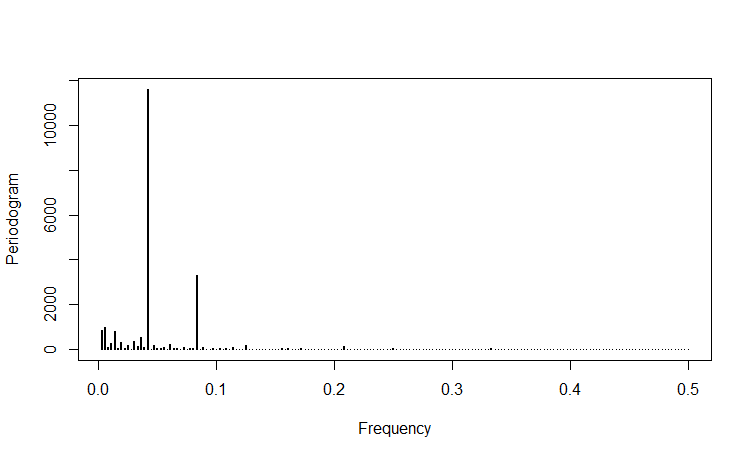
\includegraphics[width=0.8\textwidth]{figures/forecasting/periodogram_July_2014.png}
	\caption{Periodogram of hourly day ahead prices in July 2014}
	\label{fig:periodogram_July_2014}
\end{figure}


\section{Model generation}





\section{Model selection algorithm}



\section{R / Java Simulation Framework}



\section{Forecast model evaluation}





%  Generated from R function getRMSEResults: Get results from forecast simulation 
% -----------------------
% Get results from forecast simulation for the given location
% over a time range of 3 years, generate models in intervals of 1 week
% with 2,3 and 4 weeks of trainings data periods
% 5 locations are available from the forecast simulation (Application server):
%  1) Hamina, locationId 1, DA
%  2) St.Ghislain, locationId 2, DA
%  3) Portland, locationId 4, RT
%  4) Richmond, locationId 6, RT
%  5) Hatfield, locationId 8, RT






%%%  General results - all numbers  %%%


Four simulations have been run for four different locations over three years of energy price data. 
For each of these locations three different training periods have been evaluated: two weeks, three weeks and four weeks. 
Each of these simulations is evaluated for five different accuracy measures: 

\begin{itemize}
	\item Mean error (ME)
	\item Mean absolute error (MAE)
	\item Root mean squared error (RMSE)
	\item Mean percentage error (MPE)
	\item Mean absolute percentage error (MAPE)
\end{itemize}

In addition, each of these error measures has been evaluated for ten different forecast horizons (in hours): 
1, 3, 6, 12, 18, 24, 36, 48, 96, 168. 

In the tables below results are shown aggregated by forecast horizon for each accuracy measure. Each table depicts a different training period for the given location. 



\subsection{Forecast evaluation results}

% latex table generated in R 3.1.1 by xtable 1.8-2 package
% Mon Mar 07 23:15:14 2016
\begin{table}[ht]
\centering
\begin{tabular}{rrrrrrr}
  \hline
 & mean & ses & holts & holtwinters & arima & tbats \\ 
  \hline
2 weeks & 14.55 & 11.60 & 62.76 & 73.65 & 10.23 & 8.19 \\ 
  3 weeks & 14.78 & 11.60 & 62.90 & 74.02 & 9.53 & 8.59 \\ 
  4 weeks & 14.99 & 11.60 & 63.23 & 85.06 & 9.26 & 8.44 \\ 
   \hline
\end{tabular}
\caption{Results of evaluation for Hamina, Nord Pool Spot (DA)} 
\end{table}


% latex table generated in R 3.1.1 by xtable 1.8-2 package
% Mon Mar 07 23:15:14 2016
\begin{table}[ht]
\centering
\begin{tabular}{rrrrrrr}
  \hline
 & mean & ses & holts & holtwinters & arima & tbats \\ 
  \hline
2 weeks & 17.07 & 15.23 & 127.13 & 186.82 & 13.49 & 1.27E+50 \\ 
  3 weeks & 17.40 & 15.27 & 128.05 & 190.21 & 12.94 & 11.60 \\ 
  4 weeks & 17.59 & 15.30 & 127.03 & 186.37 & 12.87 & 2.49E+36 \\ 
   \hline
\end{tabular}
\caption{Results of evaluation for St.Ghislain, Belpex (DA)}
\end{table}
% latex table generated in R 3.1.1 by xtable 1.8-2 package
% Mon Mar 07 23:15:14 2016
\begin{table}[ht]
\centering
\begin{tabular}{rrrrrrr}
  \hline
 & mean & ses & holts & holtwinters & arima & tbats \\ 
  \hline
2 weeks & 24.22 & 23.61 & 235.84 & 407.06 & 24.03 & 5.45E+16 \\ 
  3 weeks & 24.14 & 23.56 & 238.92 & 686.95 & 22.26 & 1.64E+18 \\ 
  4 weeks & 24.68 & 23.32 & 268.10 & 437.85 & 21.91 & 2.18E+32 \\ 
   \hline
\end{tabular}
\caption{Results of evaluation for Portland, ISO-NE (RT)}
\end{table}
% latex table generated in R 3.1.1 by xtable 1.8-2 package
% Mon Mar 07 23:15:14 2016
\begin{table}[ht]
\centering
\begin{tabular}{rrrrrrr}
  \hline
 & mean & ses & holts & holtwinters & arima & tbats \\ 
  \hline
2 weeks & 14.47 & 15.17 & 148.54 & 322.41 & 15.03 & 7.57E+13 \\ 
  3 weeks & 14.46 & 15.23 & 147.77 & 318.61 & 14.14 & 13.46 \\ 
  4 weeks & 14.42 & 15.29 & 148.67 & 357.82 & 14.11 & 5.44E+108 \\ 
   \hline
\end{tabular}
\caption{Results of evaluation for Richmond, PJM (RT)}
\end{table}



